%\renewcommand{\ttdefault}{pcr}
%\lstset{basicstyle=\ttfamily}
%\lstset{framextopmargin=50pt,frame=bottomline}
%\lstset{language=C++}
%\begin{lstlisting}

%\begin{minted}{c++}
%GL_first_hmw.h
%#include <iostream>
%#include <math.h>
%#include <conio.h>

%using namespace std;

%//сравнения будем проводить с epsilon. Так как оно очень маленькое - то заменяем его в сравнении с нулем
%float epsilon=1.0e-7;

%void functionF();
%\end{minted}
%\end{lstlisting}

Оскільки часу було замало, а ідея нова, часу на програмну реалізацію не
вистачило.
Замість цього в даному розділі буде наведено основні ідеї та діаграми.

У підрозділі \ref{section:precedences} було наведено послідовності дій студентів
та викладачів у реальному житті.
Задача даної частини доповіді --- представлення архітектури майбутньої системи.

Розглянему діаграму на рис. \ref{fig:scheme_main}, на якій представлено загальну
структуру системи --- її компоненти та зв’язки між ними.

\begin{figure}[htbp]
    \center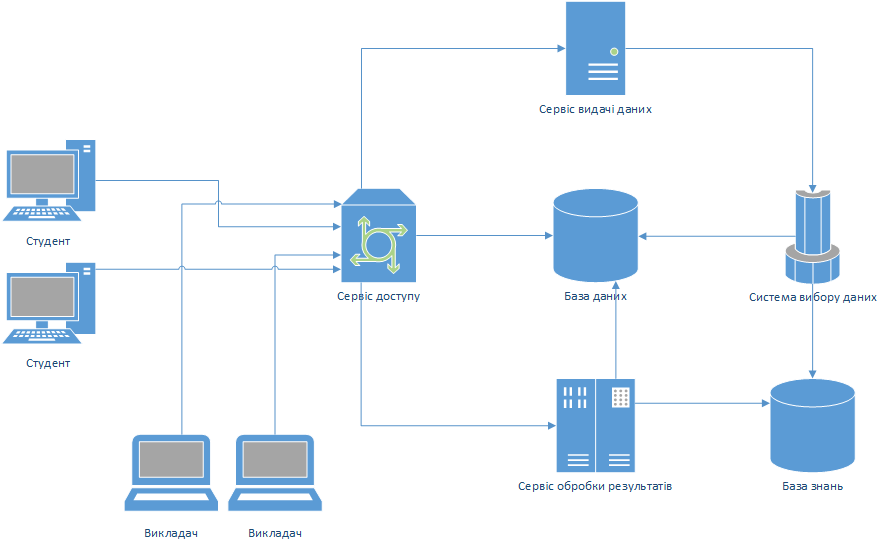
\includegraphics[width=\textwidth]{images/scheme_main.png}
    \caption{Схема роботи системи}
    \label{fig:scheme_main}
\end{figure}

Тепер подивимось на схему на рис. \ref{fig:bpmn_tests}.

\begin{figure}[h!]
    %\center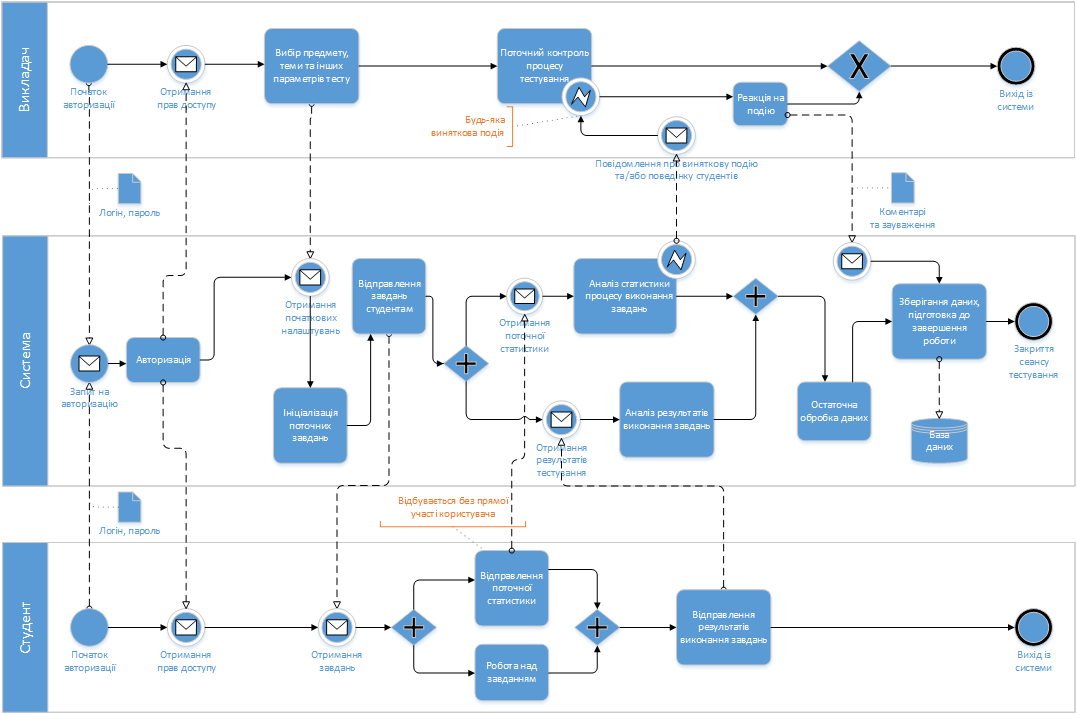
\includegraphics[height=23em,angle=90]{images/bpmn_tests.png}
    %\center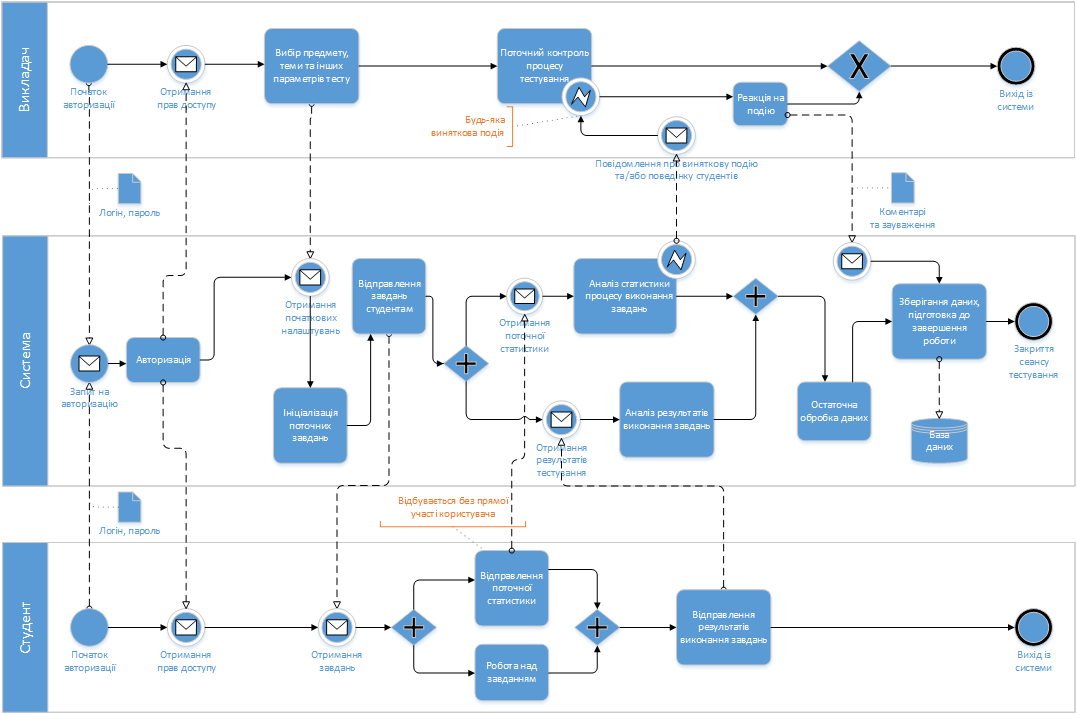
\includegraphics[width=\textwidth]{images/bpmn_tests.png}
    \center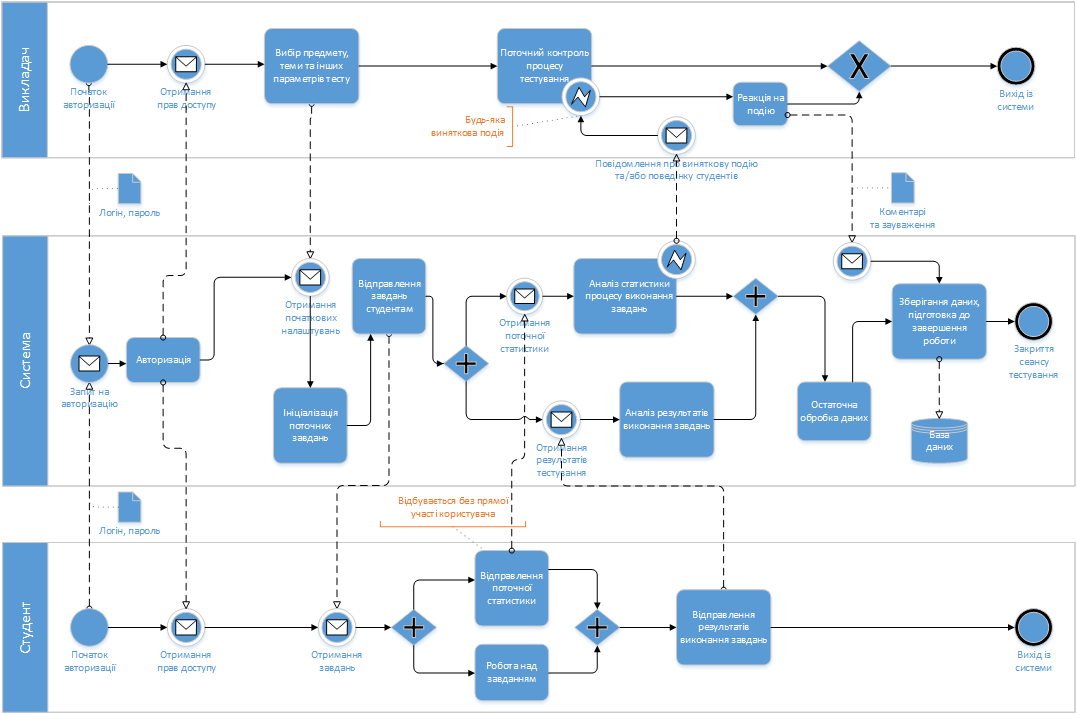
\includegraphics[height=30em,angle=-90]{images/bpmn_tests.png}
    \caption{BPMN-діаграма процесу проміжної перевірки знань,
    побудована на базі підрозділу \ref{section:precedences}}
    \label{fig:bpmn_tests}
\end{figure}

Користувачам потрібно спочатку авторизуватися, після чого студенти зможуть
отримувати завдання для виконання від відповідного сервера (сервіс видачі даних
для тестування), а викладачі зможуть отримувати від системи результати і ряд
рекомендацій щодо оцінювання.

Сервіс видачі даних орієнтується на ряд правил, серед яких частота користування
даними, використані дані в конкретній групі студентів, рівень знань конкретного
студента, рівень складності завдань тощо.
Правила націлені на покращення об’єктивності оцінювання.

Сервіс обробки результатів тестування опрацьовує результати кожного оцінювання.
При цьому відбувається як перевірка правильності виконання роботи, так і збір
різного роду статистики (час виконання як всього завдання так і окремих
підзавдань, кількість виправлень тощо), на основі якої система може
порекомендувати викладачу подальші дії: провести повторне тестування
конкретного студента, провести усне опитування (якщо студент не викликає довіри
протягом декількох спроб), змінити складність завдань або взагалі
переробити/видалити завдання.

Також можна розбити викладачів на декілька рівнів ієрархії відповідальності, де
інформація про оцінювання викладачами нижчих рівнів буде передаватися викладачам
вищих рівнів ієрархії.

Система не орієнтується на конкретний тип даних, тому можуть використовуватись
як прості тести з набором готових відповідей, так і завдання, де необхідно
написати текст пояснення, код програми, намалювати контур, побудувати діаграму
тощо.

Розглянемо схему з рис. \ref{fig:bpmn_teachers}.
Вона описує поведінку системи в режимі функціонування система-викладач.
Опустивши деталі авторизування користувачів, будемо вважати, що певну кількість
тестів успішно завершено (є тестову вибірку) і система має дані для роботи.

\begin{figure}[b!]
    \center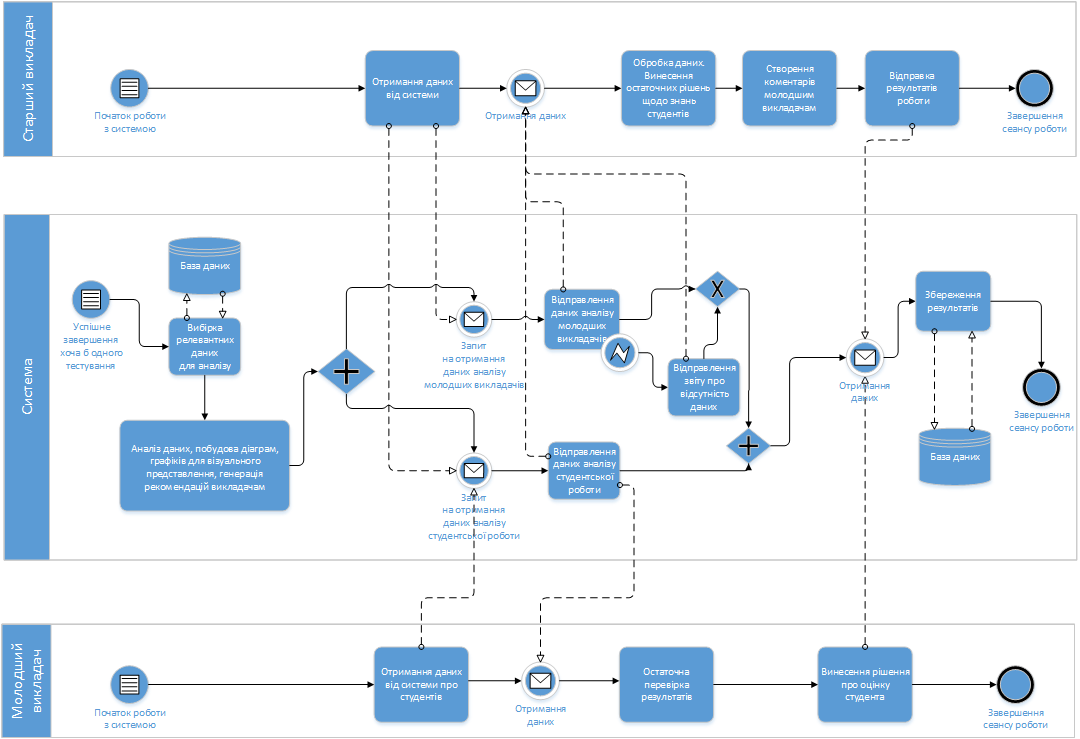
\includegraphics[height=30em,angle=-90]{images/bpmn_teachers.png}
    \caption{BPMN-діаграма процесу взаємодії викладачів і системи}
    \label{fig:bpmn_teachers}
\end{figure}

За таких початкових умов викладачі, що мають доступ до даних конкретного
курсу і групи, можуть продивлятися успішність студентів та аналізувати
статистику процесу тестування, що представлена наглядно.
На основі доступних даних викладач може змінювати оцінку студенту та
приймати рішення щодо подальшого оцінювання.

При реалізації системи онлайн тестування, тобто, в таких умовах, де студент може
здавати завдання з будь-якого місця, є доцільним реалізувати можливість
викладачу надати новий блок завдань студенту та відправити йому
повідомлення зі своїм рішенням --- в тому числі про необхідність усної здачі.

Крім того, викладач вищого рівня може контролювати оцінювання викладачів
нижчого. Наприклад, наскільки швидко завдання остаточно перевірені, наскільки
об’єктивне оцінювання та багато іншого.

Як було сказано у вступі, дана частина системи є однієї із найважливіших, бо
саме вона є базою для ідеї покращення об’єктивності навчання шляхом глибокого
аналізу різноманітних даних.
